\documentclass{standalone}
\usepackage[x11names]{xcolor}
\usepackage{tikz}

\begin{document}
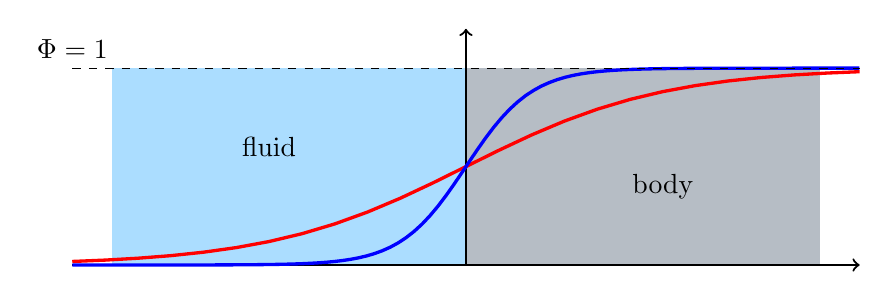
\begin{tikzpicture}[scale=2.5]
  \fill[SkyBlue1!70] (-1.8,0) rectangle (0,1);
  \fill[SlateGray4!50] (0,0) rectangle (1.8,1);
  \draw[thick,->] (-2,0) -- (2,0);
  \draw[thick,->] (0,0) -- (0,1.2);
  \draw[domain=-2:2,very thick,variable=\x,red] plot ({\x},{0.5*(tanh(\x)+1)});
  \draw[domain=-2:2,very thick,variable=\x,blue] plot[samples=100] ({\x},{0.5*(tanh(3*\x)+1)});
  \draw[-,dashed] (-2,1) node[above] {$\Phi=1$} -- (2,1);
  \node at (1,0.4) {body};
  \node at (-1,0.6) {fluid};
\end{tikzpicture}
\end{document}
